\documentclass[11pt]{article}
\usepackage[utf8]{inputenc}
\usepackage[margin=1in]{geometry}

\usepackage{graphicx}
\usepackage{algorithmicx}

\usepackage{algorithm}
\usepackage[noend]{algpseudocode}
\algnewcommand\Or{\textbf{ or }}
\algnewcommand\Init{\textbf{initialize }}
\MakeRobust{\Call}

\usepackage{tikz}
\usetikzlibrary{calc,shapes.multipart,chains,arrows,positioning}

\tikzstyle{vertex}=[draw,fill=myseagreen,circle,minimum size=24pt,inner sep=0pt]

\tikzstyle{splitvertex}=[draw,fill=myseagreen,circle split,minimum size=24pt]

\title{More Dynamic Programming}
\author{Daniel Wisdom}
\date{October 27, 2017}

\begin{document}


\maketitle



\section{Parts of a Dynamic Programming Solution}
Every Dynamic Programming solution has three parts.  Once you can write out all three parts you have a full algorithm.
\begin{enumerate}
    \item \textit{States}: A description of how the subproblems are represented.  A subproblem is usually identified by a list of one or more variables.  For example, in solving Fibonacci, a subproblem is identified by being the $i$th Fibonacci number.  The rest of the solution is then solving the subproblem for each state.   
\item \textit{Base Cases}: Base cases are simple problems which are easy to solve without any other subproblems.  In Fibonacci the two base cases are Fib(1)=1 and Fib(2)=1.  We do not need to do any deeper calculations here; Just check if $i=1$ or $i=2$ and return 1.  A poorly designed base case can lead to infinite recursion.
\item \textit{Recurrence Relation}: The recurrence relation is a method for finding the solution to a non-base case subproblem \textit{in terms of smaller subproblems}.  For Fibonacci the recurrence relation is Fib(n)=Fib(n-1)+Fib(n-2).
\end{enumerate}


\section{Examples}


\subsection{Jumping Cows}
The cows have devised a game: Every square on a sidewalk is marked with a number of points Points($i$). For every square that a cow steps in that cow gets Points($i$) points. Every turn, a cow can either move forward one space or jump forward four spaces, skipping three spaces.  Find the maximum number of points Bessie can get while going from one end of the sidewalk to the other.

\begin{figure}[h]
\centering
{
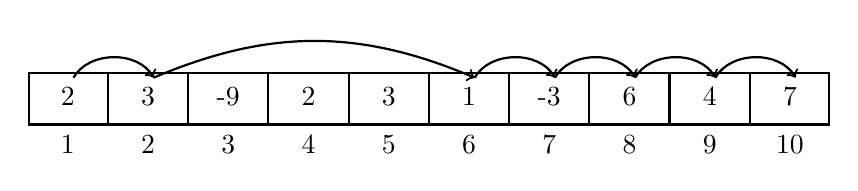
\begin{tikzpicture}[
  thick,
  myrect/.style={
    draw,
    rectangle split,
    rectangle split horizontal,
    rectangle split parts=#1,
    rectangle split part align=left,
    text width=5ex,
    text centered
    },
  mycallout/.style={
    shape=rectangle callout,
    rounded corners,
    fill=mysalmon,
    callout absolute pointer={#1},
    callout pointer width=1cm
  }  
]

\node[myrect=10]
  (array1)
  {
  					\strut 2
  \nodepart{two}	\strut 3
  \nodepart{three}	\strut -9
  \nodepart{four}	\strut 2
  \nodepart{five}	\strut 3
  \nodepart{six}	\strut 1
  \nodepart{seven}	\strut -3
  \nodepart{eight}	\strut 6
  \nodepart{nine}	\strut 4
  \nodepart{ten}	\strut 7
  };
\foreach \Valor [count=\Valori from 1] in {one ,two ,three ,four ,five ,six ,seven ,eight ,nine ,ten }
\node[below] at (array1.\Valor south) {\Valori};

\draw [bend left=60, ->] ($(array1.one)+(0.45,0.35)$) to ($(array1.two)+(0.45,0.35)$);
\draw [bend left=23, ->] ($(array1.two)+(0.45,0.35)$) to ($(array1.six)+(0.45,0.35)$);
\draw [bend left=60, ->] ($(array1.six)+(0.45,0.35)$) to ($(array1.seven)+(0.45,0.35)$);
\draw [bend left=60, ->] ($(array1.seven)+(0.45,0.35)$) to ($(array1.eight)+(0.45,0.35)$);
\draw [bend left=60, ->] ($(array1.eight)+(0.45,0.35)$) to ($(array1.nine)+(0.45,0.35)$);
\draw [bend left=60, ->] ($(array1.nine)+(0.45,0.35)$) to ($(array1.ten)+(0.45,0.35)$);

\end{tikzpicture}
}
\end{figure}
\newpage
\subsection{Jumping Cows Solution}

We want to find the maximum score possible after arriving at space 10, so let us define our subproblem to be the maximum score attainable after arriving as space $i$.  Score($i$) will denote the answer to that subproblem.  Our subproblem are identified by one variable, $i$, the index of the space.

There is only one base case here: The maximum score possible after arriving at the starting space is just the points of the start space.  Specifically, Score(1)=Points(1).

Now for the hard part: the recurrence relation.  There are two ways to arrive at a space: by moving or jumping.  A cow could get Score($i-1$) points after arriving at the previous space and get Points($i$) more point upon arriving at space $i$.  A cow could also have gotten Score($i-4$) points before arriving at space $i-4$ and get Points($i$) point after jumping to space i.  Based on these two options, the maximum number of points after getting to space $i$ is the maximum of these two possible way of getting there.  The full recurrence relation is:

Score($i$)=max(Score($i-1$) + Points($i$), Score($i-4$) + Points($i$)).
\newline

When implementing this, be careful of array out of bound exceptions.  S($i-4$) will throw errors if $i\leq3$.
We can use a bottom-up approach to the problem because:
\begin{enumerate}
    \item Every S($i$) will need to be computed, so recursion will not save any work.
    \item Calculating S($i$) only requires the results of indices less than $i$.  This means that if we calculate S($i$) starting at 1 up to 10, we will have all the information we need at every step.
\end{enumerate}

On a sidewalk with $N$ spaces, this algorithm uses the recurrence relation $N$ times, and each evaluation of the recurrence relation is O(1).  This creates a runtime of O($N$).

\subsection{Counting Paths}

Bessie the cow is navigating a complicated grid of streets to get from her house to her favorite park.  In fact, all the streets are one-way: Bessie can only move up or to the right.  To make matters worse, some of the intersections are entirely blocked.  Please find the number of unique paths which Bessie can take from her house to the park.

\begin{figure}[h]
\centering
{
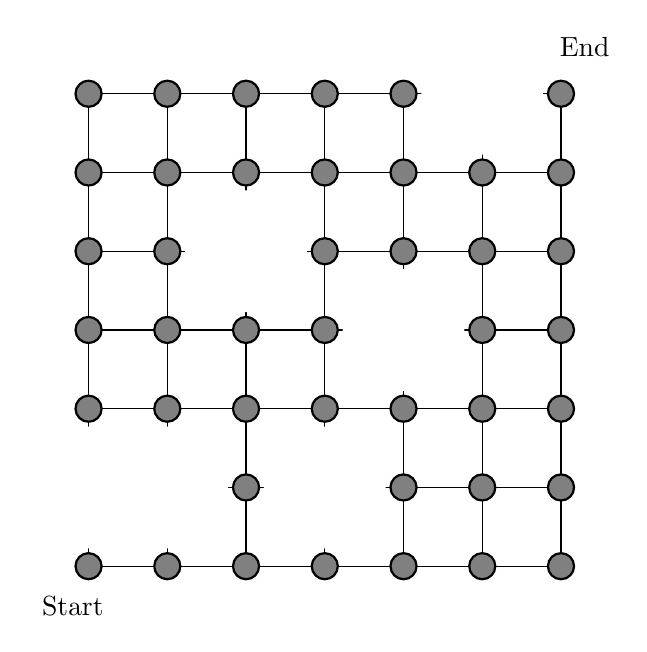
\begin{tikzpicture}[
  thick,
  myrect/.style={
    draw,
    rectangle split,
    rectangle split horizontal,
    rectangle split parts=#1,
    rectangle split part align=left,
    text width=5ex,
    text centered
    },
  mycallout/.style={
    shape=rectangle callout,
    rounded corners,
    fill=mysalmon,
    callout absolute pointer={#1},
    callout pointer width=1cm
  }  
]

\draw[step=1cm,thin] (-1,-1) grid (5,5);
\node at (-1.2,-1.5) {Start};
\node at (5.3,5.6) {End};
\foreach \x in {0, ..., 6}
    \foreach \y in {0, ..., 6} 
        \node [draw, circle, fill=gray, minimum size=2] (\x\y) at (-1+\x, -1 + \y) {};

\node [circle, fill=white, minimum size=44] (1) at (0, 0) {};
\node [circle, fill=white, minimum size=44] (1) at (1, 3) {};
\node [circle, fill=white, minimum size=44] (1) at (2, 0) {};
\node [circle, fill=white, minimum size=44] (1) at (4, 5) {};
\node [circle, fill=white, minimum size=44] (1) at (3, 2) {};
\node [circle, fill=white, minimum size=44] (1) at (-1, 0) {};
\end{tikzpicture}
}
\end{figure}

\subsection{Counting Paths Solution}

Our solution is based on the fact that if you know the number of paths to a node's two predecessors, you can easily find the number of paths to that node.

Because of this, our subproblems are the number of paths to node($x$,$y$).

Here we have two base cases: Node (0,0) has exactly one path to it.  Our other simple case is blocked intersections.  If an intersection is blocked, we know there are zero valid paths to it.

Our recurrence relation is actually quite simple too.  If the are $k$ ways to get to the node below node ($x$,$y$) and $j$ ways to get to the node to the left of ($x$,$y$) then there are exactly $k+j$ ways to get to ($x$,$y$).  The formal relation is:

paths($x$,$y$) = paths($x-1$,$y$) + paths($x$,$y-1$)
\newline

Here we have to be more careful with the order we iterate over the nodes.  We never need any information about anything above node ($x$,$y$) to find paths($x$,$y$).  This means we can fill in paths by row from bottom to top.  This same property applies to columns, so inside each row we can iterate from left to right.

On an $N$x$M$ grid, this algorithm uses the recurrence relation $MN$ times, and each evaluation of the recurrence relation is O(1).  This creates a runtime of O($MN$).

\subsection{More Advanced Path Counting}
If Bessie is willing to walk the wrong way on up to one road per trip, how many paths are there to the park now?  This means that Bessie can move left or down once or never during her trip.  For example if Bessie legally got to the park, but then walked down one block and back up again, that would count as a unique path.

\section{Problems}
\begin{enumerate}
\item \textbf{Coin Change.} Given $n$ types of coin denominations with values \texttt{V[0]}, \texttt{V[1]}, \dots, \texttt{V[n-1]}, determine the minimum number of coins needed to make change for an amount of money $C$. Assume \texttt{V[0] = 1} so that you will always be able to make change for any amount $C$.
\item \textbf{Knapsack Problem.} You have a bag that can hold weight $Wmax$.  There are N different types of items, each having a value V[$i$] and weight W[$i$].  What is the highest value you can fit in your bag and keep the sum of the weights less than or equal to $Wmax$.  You may take as many of any item as you can fit.
\item \textbf{0/1 Knapsack Problem.} This is like the Knapsack Problem, but you can take either 0 or 1 of each item.
\end{enumerate}
\end{document}

